\documentclass{%
	article}
\usepackage[utf8]{inputenc}

\usepackage{url}
\def\UrlBreaks{\do\/\do-}

\usepackage{graphicx}
\usepackage{amsmath}
\usepackage{verbatim}
\usepackage{seqsplit}
\usepackage[table,xcdraw]{xcolor}
\usepackage{blindtext}
\usepackage{listings}
\usepackage{color}
\usepackage{titling}
\usepackage[T1]{fontenc}
\usepackage{authblk}
\usepackage{flafter}
\usepackage{here}

\usepackage{tabularx,booktabs,ragged2e}
\newcolumntype{C}{>{\Centering\arraybackslash}X} % centered "X" column

\usepackage[labelfont=small]{caption}

\lstset{frame=tb,
  aboveskip=6mm,
  belowskip=6mm,
  showstringspaces=false,
  columns=flexible,
  basicstyle={\small\ttfamily},
  breaklines=true,
  breakatwhitespace=true,
  tabsize=4
}
\renewcommand\lstlistingname{Algorithm}

\title{The Hadron Cryptographic Ledger Project: a framework for the rapid development\\and deployment of blockchain technologies.}
\author{Stuart Farmer\thanks{stu@hadronledger.com}}
\author{Mario Hernandez\thanks{mario@hadronledger.com}}
\author{James Munsch\thanks{james@hadronledger.com}}
\affil{The Hadron Project, White Paper version 0.1}

\begin{document}
\sloppy

\begin{titlingpage}
    \maketitle
    \begin{abstract}
	Blockchain application development is unnecessarily hard, partially because of how new the technology is, but also because of certain imposed limitations on the current status quo of how blockchains are used today. In this paper, we discuss the problems with current blockchain implementations and a solution to these problems. We introduce Hadron: a software package of development tools that includes a blockchain generator, community collaboration tools, and independent chain-to-chain communication to create vast networks of blockchain applications that can transfer any asset across them.
    \end{abstract}
\end{titlingpage}

\section{Motivation}

In the past several years, we have seen an influx of blockchain technologies hitting the market. These technologies are touted as a means to an end of the centralized banking and financial systems. However, these blockchains rely on flawed systems that do not take into account the application of said technologies into the current infrastructure space. As a result, blockchain technology is segregated from the mainstream financial systems, and thus is ironically hindered by achieving its end goal.

The Hadron project is an effort to create software development tools that increase the mass adoption of blockchain technology so infrastructure can revolutionize the market systems and cause realistic innovation within the markets.

Laid out in this white paper is our critiques of the current state of the markets, and how we plan on improving this space.

\section{Problems with Current Blockchain\\ Implementations}

There are many fundamental flaws with the blockchain architecture that prevent it from becoming a mainstream technology. These flaws exist on both the user’s side as well as the developer\,/\,service provider’s side. Laid out are the areas in which we improve upon the current blockchain implementations with this project.

\begin{center}
\textbf{Transaction Fees}
\end{center}

Firstly, let’s take a look at the problem with transaction fees from an end user standpoint. The key to success in the crypto space is mass adoption of Bitcoin in the international market. As it stands at this time of writing, the average transaction fee for a Bitcoin transaction is at around 6\%\,\cite{bitcoinfees}. Compared to centralized systems such as PayPal\,\cite{paypalfees}, Mastercard\,\cite{mastercardfees}, and Visa\,\cite{visafees}, Bitcoin is actually about twice as expensive.

It should be noted the fundamentals of cryptocurrency are why users feel justified with this discrepancy. The decentralized nature of ownership outweighs the additional costs. However, on a macroeconomic scale, cost efficiency will outweigh fundamental allure.

\begin{center}
\textit{“But what about Ethereum? Their transaction fees are only 0.3\%!”}
\end{center}
	
While this is true, the Ethereum blockchain was not designed as a transfer of value network\,\cite{ethereumwp} like Bitcoin was, but rather a smart contracts network to enable trustless and decentralized software systems. We have to remember that users instead pay for the number of operations that occur on the chain and that this number of operations continues to increase as more and more complicated smart contracts are deployed. A major selling point of Ethereum was the ability to add smart contracts as ‘libraries’ that function in the same way as frameworks in other software development stacks which is to automate operations and processes so users do not have to rewrite them over and over again. Thus, we can safely assume that over time, as more complex smart contracts are made and more libraries are integrated, the cost of interacting with the main Ethereum blockchain. This mechanism by charging developers on operations disincentivizes innovation and complex smart contract systems that Ethereum needs to be a long term success.



\begin{figure}[htbp!]
\centering
\resizebox{\textwidth}{!}{%
\setlength\extrarowheight{2pt}
\begin{tabularx}{\textwidth}{l X l}
\toprule
\textbf{Service Name} & \textbf{Average Transaction Cost}                                                                                         & \textbf{Paying Party} \\ \cmidrule[\heavyrulewidth]{1-3}
Bitcoin\,\cite{bitcoinfees}			& {\small{$\sim$}}6\% (variable) & Sender \\ \midrule
PayPal\,\cite{paypalfees}			& 2.9\% + \$0.30 & Receiver \\ \midrule
Visa\,\cite{visafees}				& Based on merchant type. As low as 0.20\% for utility payment, to as high as 1.50\% for standard merchants. & Receiver \\ \midrule
Mastercard\,\cite{mastercardfees}	& Based on merchant type. As low as 0.00\% + \$0.65 for utility payment, to as high as 2.95\% + \$0.10 for standard merchants. & Receiver \\ \midrule
Stripe\,\cite{stripefees}			& 2.9\% + \$0.30 & Receiver \\ \bottomrule
\end{tabularx}%
}\par
\medskip
Table 1: Various payment services and their transaction costs.
\end{figure}


\begin{center}
\textbf{Bloated Chains}
\end{center}

Carrying on with the Ethereum model, because the ledger is public, anyone can deploy whatever smart contracts they’d like. As a result, even though the blockchain is only two years old, the size of a full node is 242GB\,\cite{ethchainsize}, which is even larger than the current size of a Bitcoin full node which is around 152GB\,\cite{btcchainsize}. Having to install a full node, or at least a light chain which is still around 20Gb of data, is a hefty barrier of entry for someone who just wants to dabble in smart contract development.

Compare the time it takes to fully sync a node with the time it takes to install Python, Node.js, or any other programming environment to start poking around. The inconvenience and download size alone are unfeasible to most developers and companies, let alone the average user who is curious about blockchain technology.

\begin{center}
\textbf{Transactions per Second (Scalability)}
\end{center}

Modern blockchains have a notoriously low throughput rate which causes transaction times to be slow, and a backlog of pending transactions to pile up. This is an unacceptable replacement for the current financial systems that process millions of transactions per day.

For example, Bitcoin has a throughput rate of 3 transactions per second. Likewise, Ethereum boasts a mere 15 transactions per second\,\cite{transactbandwidth}. In comparison, PayPal released a case study in May of 2015 where they were able to create a system throughput rate of over a billion transactions a day. That translates to about 11,600 transactions per second\cite{paypalcasestudy}.

This disincentivizes enterprises that deal with assets in a traditional high throughput database structure to sacrifice capacity for the benefits of high record maintenance.

\begin{center}
\textbf{Mining and Resource Efficiency}
\end{center}

Another barrier towards mass adoption is the arbitrary hashing functions that mining rigs perform to ‘prove work.’ These machines take up massive amounts of resources in energy costs that make no sense to the standard enterprise user. Whereas this is an approach to distributing tokens and coins on a main chain, it does not translate to the business setting where capital resources are optimized. Inefficient processing makes no sense to the modern business, and thus these types of pointless hashing functions are impeding widespread adoption.

\begin{center}
\textbf{Integration and Adoption}
\end{center}
Blockchain software is very new and the human capital resources are scarce. It requires a very highly technical and specialized individual to consult and develop for blockchain applications. Compared to other database types in a corporate setting, setting up a blockchain is time consuming and expensive. 

Whereas most modern database systems follow a similar development and deployment paradigm, blockchains are so fundamentally different that there is currently not a solution in place to transforming the development process into something that resembles other database systems on the market.

Furthermore, development environments, package managers, testing suites, continuous integration environment, etc. which exist for nearly every other tech stack in existence do not exist for blockchain software. This prevents organizations from integrating this technology into their current workflow.

\begin{center}
\textbf{Migration, Upgrades, and Future Proofing}
\end{center}

For many interested in blockchain technologies for their enterprises or businesses, the lack of ability to migrate data to a new chain, or to upgrade at a time that is best for a business is a pitfall. Those interested in mainchain and public ledger systems are reliant on foundations to release new code or the decentralised community where there is little authority or certainty to the outcome. Furthermore, trying out different systems to see what works best for an organization is cumbersome.

\section{The Solution}

The Hadron project proposes the creation of a suite of development tools that allows rapid development and deployment of private blockchain systems that mimics the modern development process featured in such tech stacks as Node.js or Python which provide a plethora of easy to use tools, extensive and robust documentation, and vastly popular support communities.

The project is broken up into three sections, the Hadron Wrapper, the Hadron Hub, and the Hadron Ledger, which each add a layer to end goal of providing hyperfast blockchains for developer to test, experiment, and deploy across a network of other blockchain systems.

The Hadron Wrapper is the generator tool to deploy private chains on an internal network without any hassle. The Hadron Hub is a central repository for smart contract packages and templates, private chain naming services, and blockchain discovery. The Hadron Ledger is the network that handles payment channel swap processes between chains and facilitates communication between blockchain apps on the network in a way that remains trustless and decentralized.

\begin{center}
\textbf{The Hadron Wrapper}
\end{center}

Instead of having a single mainnet which suffers from the problems mentioned above, breaking up blockchains into individual use cases and having them interact with each other when needed solves many problems with low blockchain adoption rate. For example, an organization would have their own blockchain for their own web app. This allows them to have complete control over the technology that they use as well as dedicating their own computing resources to running that blockchain, rather than wasting effort on a main chain. Furthermore, ‘gas’ in the case of an Ethereum chain can be eliminated and the difficulty of a network can be turned down to a more reasonable level, thus enabling free transactions across their application. This makes a blockchain act more like a web server than a traditional chain and can then be used to replace and upgrade existing database structures internally.

\begin{center}
\textbf{Motivation for Independent Consensus}
\end{center}

What makes blockchain technology work is the fact that miners are independent actors that verify transactions that occur so it is near impossible to inject false information into the chain. However, in traditional settings, miners are rewarded in cryptocurrency from transaction fees. Because transactions are free on the Hadron protocol, a different rewarding mechanism must be instilled so that miners are still motivated to provide independent verification of transactions.

It is possible to create proof-of-work, proof-of-stake, and any other rewarding schemes by using smart contracts. In this way, a smart contract can be called upon to calculate the reward and recipient, and reward any type of asset on the chain. Instead of just the native currency of the chain (which is initially Ether), ERC20 tokens or novel cryptoasset implementations can be rewarded as well, providing even more customization to private chains. And because transactions and gas is free on the networks, calling a contract one a block, for example, is not expensive.

\begin{lstlisting}[
	belowskip=1mm,
	title={\small\textnormal{Listing 1: Example of a simple proof-of-work contract that could be deployed on a chain to simulate classical proof-of-work.}},
	captionpos=b]
pragma solidity ^0.4.15;

contract RewardedAsset {
    string public constant symbol = "AU";
    string public constant name = "Digital Gold";
    uint8 public constant decimals = 0;
    uint256 _totalSupply = 1000000000;
    uint8 public reward = 10;
    uint256 lastBlock;

    address public owner;
    mapping(address => uint256) balances;
    mapping(address => mapping (address => uint256)) allowed;

    function disperseRewards (bool success) onlyOwner() {
        if (lastBlock < block.number) {
            _totalSupply += reward;
            balances[block.coinbase] += reward;
            lastBlock = block.number;
        }
    }

\end{lstlisting}

\begin{center}
\textbf{Generator Tool}
\end{center}

The Hadron Wrapper is taking design queues from other package management CLI (Command-Line Interface) tools such as \texttt{pip}\,\cite{pip}, \texttt{yeoman}\,\cite{yeoman}, and \texttt{npm}\,\cite{npm} to generate private blockchains as their own development projects. Generation through the CLI took is as simple as ‘\texttt{hadron init}’. Through this CLI application, you will be able to interact with the chain in a simplified API that abstracts most of the complexities of blockchain technologies from you.

The initial blockchain technology that we are implementing is Ethereum, and so developers will be able to initialize these chains, create accounts, mine blocks, and deploy contracts in a sub-processed instance of \texttt{geth}, Ethereum’s client written in Go.

By abstracting the main interaction components away from \texttt{geth} into a CLI tool, we are able to then provide a RESTful API service for interacting with these private chains. A RESTful API allows for blockchains to be interacted with across the Internet in literally any programming language interface. If a programming language supports HTTP requests, they will be able to interact with Hadron generated private chains. This allows integration into any tech stack, and allows us to create drop in libraries for many modern language frameworks such as Swift for iOS development, Java for Android development, and even embedded C for Internet of Things applications.

Furthermore, the Hadron Wrapper will provide a local server with an Ethereum blockchain explorer that can be public facing so that the wider community can monitor and see the activity occurring on the chain.

A web service to manage the chain from a graphical web interface similar to Parse will also be included out of the box.

Optionally deployable instances of IPFS\,/\,IPNS and Tor.

\begin{center}
\textbf{Deployment}
\end{center}

After the development of a private chain, an organization will want to package and deploy that in a way that can integrate into their internal technical stacks. To do this, the Hadron Wrapper will export Docker files for quick deployment.

\begin{center}
\textbf{Architecture}
\end{center}

Beyond creating a private chain instance, the Hadron Wrapper contains the necessary methods needed to accept payment channel transactions and interact with the larger Hadron chain. Thus, the Hadron Wrapper should be thought of as a type of interface. Each Hadron Wrapper instance must adequately conform to a set of monitoring and interaction protocols to guarantee that the chain is trustless and that transactions can be independently confirmed.

If the Hadron Wrapper component can achieve these functionalities, then the internal blockchain driver does not have to be based off of Ethereum. Into the future, the Hadron Wrapper will support arbitrary blockchain technologies such as Bitcoin, Litecoin, Zcash, Monero, Neo, Tezos, Eos, and more as long as they can support payment channels in a trustless fashion. Even novel blockchain technologies that adhere to the wrapper protocol will be supported, creating a completely custom blockchain-to-blockchain interfacing network.

The Wrapper will ultimately support any blockchain technology as long as it adheres to certain specifications so that it can interact with the Hadron Ledger. This futureproofs the Hadron system so that no matter what technologies exist in the future, there will always be a network to interact with them. This also solves the problem of blockchain migration, as businesses, enterprises, and applications can upgrade to the latest blockchain projects and technology as they come out to keep ahead of the competition.

\begin{center}
\textbf{The Hadron Hub}
\end{center}

Apart from simple blockchain generation, the main driver of technology adoption is not the base use cases of the core tech, but rather the surrounding communities and feature-sets built by them. You can see this with the Ethereum community, and more with newer smart contract systems that are starting to spur innovation. Their cryptocurrency mechanisms are not what sets them apart from Bitcoin or Litecoin. Instead it is the development community surrounding and developing smart contract applications that affords wider adoption.

Similarly, package repositories that allow users to pull in packages from the wider community, comment on them, and even develop for them solidifies a base of intellectual capital that leads to the success of the project and greater innovation in the field.

The purpose of the Hadron Hub is to host a decentralized package repository, namespace system, and discovery tool so that developers of Hadron chains can connect with other developers, play off each other's innovations, and lead to a greater state of cryptocurrency.

\begin{center}
\textbf{Public Package Manager}
\end{center}

\begin{lstlisting}[
	aboveskip=1mm,
	belowskip=1mm,
	title={\small\textnormal{Listing 2: Example of a Solidity Template for ERC20 tokens with corresponding JSON input. Installation of such contract could be accomplished via ‘\texttt{hpm install erc20 --args}’, or from the Hadron Wrapper administration panel.}},
	captionpos=b]
pragma solidity ^{{solidity_version}};

contract {{contract_name}} {
    string public constant symbol = "{{symbol}}";
    string public constant name = "{{asset_name}}";
    uint8 public constant decimals = 18;
    uint256 _totalSupply = {{total_supply}};

    address public owner;
    mapping(address => uint256) balances;
    mapping(address => mapping (address => uint256)) allowed;
   
    
...


{
    'solidity_version':'0.4.15',
    'contract_name':'Testcoin',
    'symbol':'TST',
    'asset_name':'Testcoin',
    'total_supply':'1000000'
}
\end{lstlisting}

Like other development suites, Hadron has the ability to create smart contract packages. Using a macro templating system, we are able to abstract common Solidity contract types such as ERC20 tokens, Ethereum Name Services, and the Etherdelta decentralized exchange, package them up into contracts that only take a set of arguments, and allow deployment across private chains in as simple as a manner of running ‘\texttt{hpm install ens}’ from a CLI console, or sending an API request to do the same through the administrative dashboard included in the Hadron Wrapper. This takes the headaches out of redeploying commonly used smart contracts, and allows the packaging of highly complex smart applications for quick distribution.

As more blockchains are added to the Wrapper, support for their contract languages will be added to the Hub as well. Developers can upload their own contracts to support the community. Interaction with the Hub will be over the Interplanetary File System (IPFS) so that all services remain distributed and decentralized.

\begin{center}
\textbf{Name Directory Service}
\end{center}

Chains will have to communicate with one another to execute payment channels. To do this, a naming service must be implemented. This naming service assigns a common name and a key pair to each chain so that other chains can discover them and sign transaction requests to them.

Furthermore, users will be able to search and discover new blockchain applications. These are private chains developed with the Hadron Wrapper that have connected to the Hadron Ledger. Each of these chains will be able to register for a name and fill out a profile about their service which can include links to marketing sites, connection information for miners, and anything else that would lead users to more valuable information about their service. That name will be used to locate and send information to through the Hadron Ledger for payment transactions, interaction with the chains, and the general use of the native Hadron token.

We have also been exploring options in using the Token for other developers to be able to register their modules to which usage metrics could generate token liquidity between members of the developer community.

\begin{center}
\textbf{The Hadron Ledger}
\end{center}

The main technological feat of the Hadron project is its cryptographic ledger and routing system that connects private chains together. By instead of recreating an entirely new chain and instead shifting focus towards distributed private chains only tied together by a routing infrastructure, we can avoid blockchain bloat, the need to ‘sync’ with the network before interacting with it, increasing transaction costs, and guarantee a future-proof platform that will last years regardless of the further improvements upon general blockchain technology.

\begin{center}
\textbf{Routing}
\end{center}

The Hadron Ledger is primarily the infrastructure that links private chains together over a common protocol, much like a telephone network. The Ledger takes care of interaction between all chains and provides a common set of interface options to that chains can be treated the same ways in computer programming environments and platforms for further integration away from the Hadron Hub.

A main value add of the Hadron Ledger is the absence of transaction fees. In exchange for the benefits of connection to the Hadron Hub and exposing a private chain to the wider community which increases public adoption, a private chain dedicates a certain amount of computing power to the ledger overall. Because the ledger is absent of difficult hashing functions, and serves merely as an intermediary to process packets of information between chains. The computing load to connect and serve information is comparable to a modern day web server rather than a standard blockchain miner. Blockchain application providers expose a single public entry point onto the IPFS and distributed computing cluster for incoming transactions, and connect to the public Ledger node for outgoing transactions.

\begin{center}
\textbf{Payment Channels for Cross-Chain Transactions}
\end{center}

While retaining a trustless and decentralized system, it is required for a system of cross-chain payments to exist so that blockchain applications can interact with each other freely. This is the main draw of the Hadron Ledger. To do so, the Ledger implements Lightning Network\,\cite{lightning} inspired payment channels to provide a secure and decentralized method of exchanging funds across blockchains. Transactions initiate from private chains, and utilize the Ledger as a public service for managing secure and guaranteed remittance of funds from chain to chain.

The Ledger is a public service that distributes the work of smart contract deployment and identity verification for chain to chain transfers between participants connected to the main network. Private chains are free to implement their own methods by which to transfer funds to each other, but the public Ledger is verifiable by consensus of participants on the wider network, thus providing a stronger sense of trust to cross chain transactions.

Payment channels are represented in pure Solidity smart contract code that run on each private blockchain. When a user wants to initiate a swap, they send a request both the Hadron Ledger service and the chain they want to swap with outlining the terms of their expected transfer. The request is comprised of the sender and receiver address on both chains, as well as the value of the asset being swapped. For example, a payload would look like this:

\begin{lstlisting}[
	belowskip=1mm,
	title={\small\textnormal{Listing 3: Example of the payload from a payment channel.}},
	captionpos=b]
{
    Private-chain-1 : {
        Sender-address : 0x000,
        Receiver-address: 0x000,
        Amount: 100,
        Token-contract-address (optional): 0x000
    }
    Private-chain-2 : {
        Sender-address : 0x000,
        Amount: 1000,
        Token-contract-address (optional): 0x000
    }
}
\end{lstlisting}

When the computing cluster receives this payload, the cluster will compile the Solidity contract code into bytecode that must be deployed onto each chain within the next block. The opposing chains’ bytecodes are sent to each other and signed with a public identifier key so that they can independently verify that the correct contract code was indeed deployed in the next block on the chain.

\begin{figure}[H]
\centering
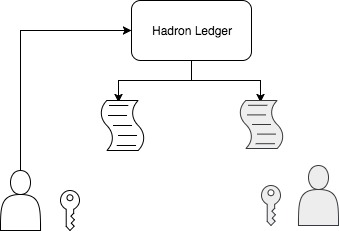
\includegraphics[scale=0.45]{fig1.jpg}
\caption{\small\textnormal{Chain A initiates a swap by sending a message to the Ledger. The Ledger then takes the swap requirements and compiles them into Solidity bytecode to be deployed on each chain.}}
\end{figure}

\begin{figure}[H]
\centering
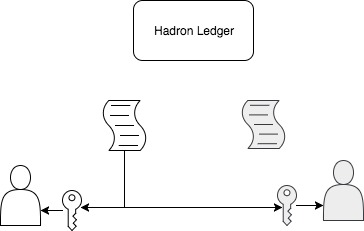
\includegraphics[scale=0.45]{fig2.jpg}
\caption{\small\textnormal{The bytecode is signed with each chain's public key and sent to both parties. Chain A deploys their contract. Chain B keeps a copy to verify later.}}
\end{figure}

\begin{figure}[H]
\centering
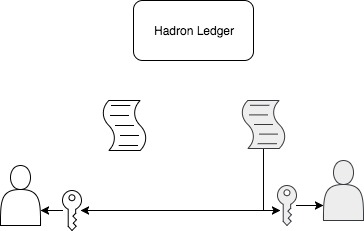
\includegraphics[scale=0.5]{fig3.jpg}
\caption{\small\textnormal{The same occurs for Chain B.}}
\end{figure}

\begin{figure}[H]
\centering
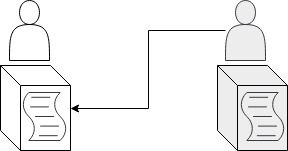
\includegraphics[scale=0.5]{fig4.jpg}
\caption{\small\textnormal{Assuming that this is an agreeable swap, both chains deploy the contract, and check to see if the other party has done the same by searching for the bytecode on the latest block. If this has not occurred, the chain does not have to follow through with any obligations, and the transaction reverts without loss of funds.}}
\end{figure}

If the originator chain fails to deploy their contract while the recipient chain follows through, the contract on the recipient chain will self-destruct and remit funds back to their account. On the flip side, if the originator sets up a contract, but the recipient does not agree to the terms, the originators contract will be destroyed they will receive their locked up funds. 
	
Assuming that both parties are interested pursuing the swap, they must then follow through with the agreed upon obligations on each others’ chains, which executes the payment channel regularly.

To make sure that the payments have been sent through in a timely fashion, each chain can ‘ping’ their contracts which invokes a time lock method. If the contract is too many blocks behind the agreed upon time lock, it is assumed that the other party is not going to finalize the payment channel, and the contract is destroyed. This incentives the opposing party to follow through with their obligations because they risk losing their funds. It also incentives the originator to ping their contract as soon as possible, because in the situation where the originator has received funds on the opposing chain but not on their chain, they can remit their funds back to themselves and in effect have gained ‘free’ assets on the opposing chain because the time lock had expired on their own to claim the assets.

\begin{figure}[H]
\centering
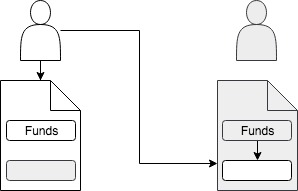
\includegraphics[scale=0.5]{fig5.jpg}
\caption{\small\textnormal{Chain A's best economic option is to submit the funds and resolve their own contract as soon as possible, because if Chain B acts before them, Chain A will lose funds. Inversely, Chain A could also profit if Chain B decided not to redeem their funds. So it is also in Chain A's best interest to resolve their contract as soon as possible}}
\end{figure}

\begin{figure}[H]
\centering
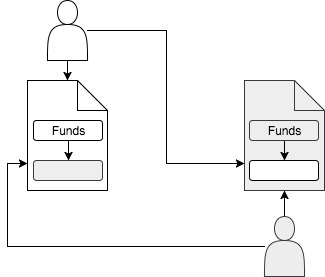
\includegraphics[scale=0.5]{fig6.jpg}
\caption{\small\textnormal{The best case scenario for both parties, therefore, is to resolve the payment channel on the opposing chain, and resolve the contract on their own chain as soon as possible. By adding economic incentive to do this, the network benefits from quick chain-to-chain transfers.}}
\end{figure}

\section{Example Workflow}
Firstly, you will install the Hadron Wrapper tool designed for developing blockchains. You will run \texttt{hadron init} inside of a project directory and generate a chain. From there, you'll install the packages you need for your application using the Hadron Hub, or our package manager named 'flora.' Let's say you want to add a new ERC20 asset. Run \texttt{flora install erc20} inside of the project directory, and a new token will be generated. To deploy the contracts to the chain, run \texttt{hadron start}, and then \texttt{hadron deploy all}.

From there, you can access the administrative dashboard if you want to graphically interact with your blockchain. You can install packages from here, add accounts, see transactions, etc. etc. much like Etherscan or another block explorer software. You will also have Remix and other smart contract development tools here as well.

From this backend, you can upload new contracts that you develop to the Hadron Hub. You can also connect your chain to the Hadron Ledger to interact with other blockchain applications. To do this, you will host an IPFS node and connect to the distributed computing cluster as a server. You can then interact with other independant blockchains as a user, or to intiate chain-to-chain swaps. You can initiate swaps with the native Boson token out of the box with all blockchains.

Now, you can integrate your other software on top of the blockchain such as a public facing user interface, automatic transfers between chains, smart contract interaction, and even interacting with custom contracts that you deploy on other chains on the Hadron Ledger. All is possible with the Hadron Project.

\begin{center}
\textbf{Maintaining Distributed and Trustless System Architecture}
\end{center}

While private chains on Hadron are built off of Ethereum which is a distributed and trustless protocol, the rest of the Hadron systems could be developed using standard centralized server-client architecture. However, while this is potentially an easier method of execution, standard HTTP protocol is vulnerable to DDOS attacks, server failure, and centralized ownership of data that sacrifices the rights of the collaborators of the project.

Thus, the project will be deployed upon the IPFS protocol to establish a true peer to peer system that is distributed and trustless.

\begin{center}
\textbf{Bosons, an agnostic digital currency}
\end{center}

While payment channels across private chains will help facilitate app-to-app communication, there should also be away for users who are involved in the Hadron project apart from a chain host or developer to easily participate and use the blockchain applications on the Hadron Hub. Thus, we propose an agnostic unit of currency known as a ‘Boson’. Bosons are a digital currency that serve the universal asset of the platform itself, available for trade by users of the system who want to use a currency that use all private chains. Communication with the Boson chain comes out of the box for Hadron developers, so they do not have to form independent relationships with other private chains to start transferring assets to one another. In this fashion, developers can start to integrate a digital currency market and trade into their blockchain applications immediately. By offering a native digital currency out of the box to all Hadron users, Bosons increase the adoption rate of private chains, as more individuals are able to participate with the application coming from the Hadron community.

\begin{center}
\textbf{Token Sale (Token Scattering Event)}
\end{center}

The Hadron project will be funded by a Token Distribution Event (Token Scattering) of the Bosons. These Bosons will be available for purchase on the Ethereum main chain in the form of an ERC20 token. Said Bosons will then be available for swapping onto the Hadron chain during a ceremonious process which signifies the milestone achievement of chain-to-chain communication on the Hadron Ledger.

Further detailing on the Token Scattering Event is included in organizational documents.

\section{Conclusion}

The goal of the Hadron project is to provide a suite of tools that makes the rapid development and deployment of blockchains easy for the general population of developers. By modelling our tools based on the most popular tools used by developers today, we can capture a large and enthusiastic base of developers who want to get involved in blockchain but are unable to get over the initial hurdles.

Furthermore, by providing a centralized community, innovation can prosper and build upon itself, leading to newer and greater technologies and accelerating the industry as a whole.

Lastly, through the Hadron Ledger, we are able to connect all of these projects together on a single routing system that facilitates swap transactions so that private chains can retain the benefits of self-management and still take advantage of a larger ecosystem of great applications.


\bibliography{references}{}
\bibliographystyle{ieeetr}

\end{document}
